\begin{figure*}[h!]\centering
\captionsetup{width=0.85\linewidth}
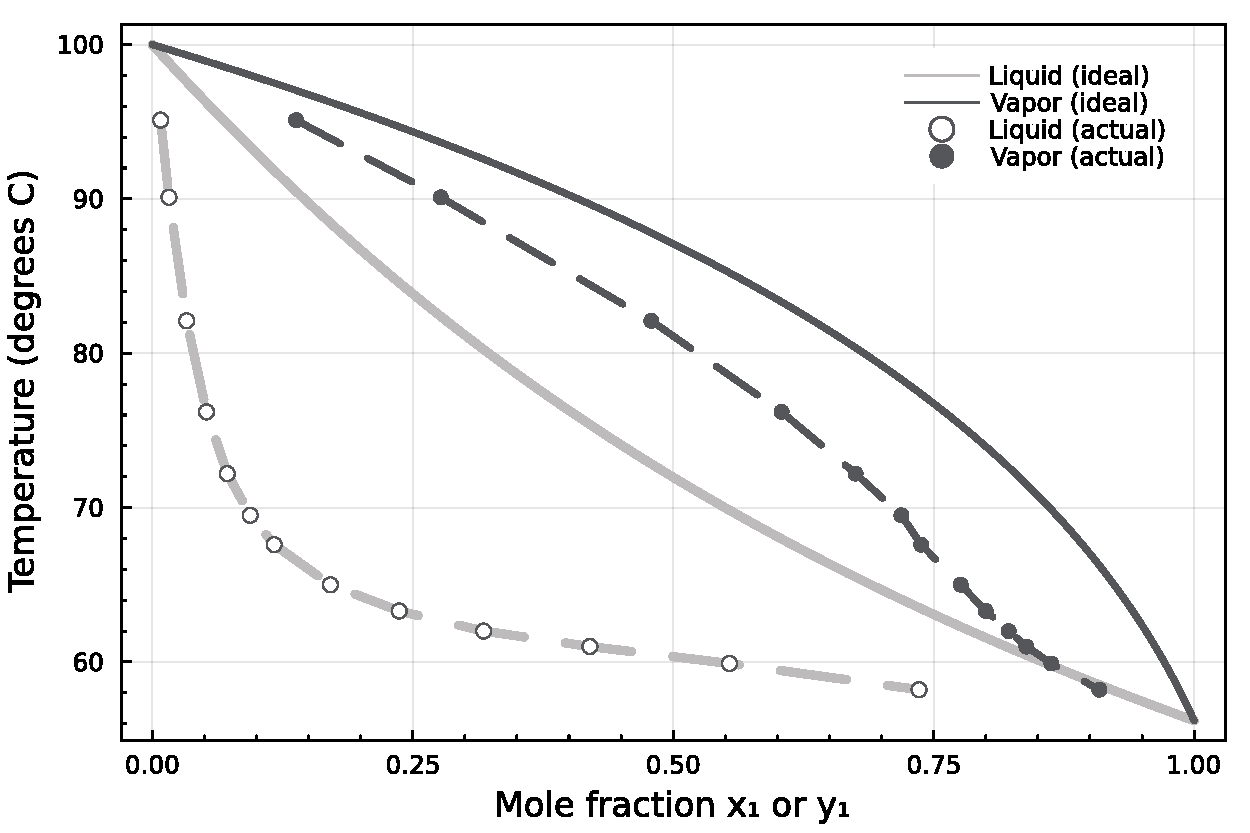
\includegraphics[width=0.85\textwidth]{./figs/Fig-Txy-acetone-water-ideal-P101_325-kPa-AP2.pdf}
\caption{Temperature ($^{\circ}C$) versus composition (x$_{1}$ or y$_{1}$) for a binary mixture of Acetone(1)/Water(2) computed assuming ideal 
liquid and vapor phases (solid lines) and measured experimentally (dashed lines).}\label{fig-VLE-ideal-problem-Txy}
\end{figure*}

\item{(25 points)
Cornell Inc. was hired to design a flash separation process for a binary ($\mathcal{M}$ = 2) mixture of Acetone(1)/Water(2).
The engineering team performed initial design calculations assuming an ideal liquid and vapor phase, a drum temperature of T = 70$^{\circ}$C and z$_{1}$ = 0.64
(Fig. \ref{fig-VLE-ideal-problem-Txy}). 

Let the saturation pressure of component $i$ be described by the Antoine equation:
\begin{equation}
  \ln\left(P_{i}^{sat}\right) = A_{i} - \frac{B_{i}}{C_{i}+T}
\end{equation}where $P_{i}^{sat}$ has units of kPa and the temperature $T$ has units of $^{\circ}C$.
The Antoine parameters are given by:

\begin{table}[!ht]
  \centering
  \caption{Antoine parameters for the Acetone/Water flash problem.}
  \setlength{\tabcolsep}{18pt}
  \begin{tabular}{c|c|c|c}\toprule
    Species & A & B & C \\ \toprule
    Acetone & 14.31 & 2756.22 & 228.06 \\
    Water & 16.39 & 3885.7 & 230.17 \\\bottomrule
  \end{tabular}
\end{table}

\textbf{Assumptions}: (i) the Flash drum operates at steady-state;
(ii) vapor-liquid equilibrium occurs everywhere inside the drum at some (T,P);
(iii) treat both the vapor and liquid phases as ideal (unless using experimental data);
(iv) the Flash drum is well-mixed;
(v) a single liquid feed (stream 1) enters, and a vapor (stream 2) and liquid (stream 3) exit the drum;
(vi) R = 8.314 L kPa K$^{-1}$ mol$^{-1}$.

\begin{itemize}
    \item[a)]{(2 points)~Using the ideal data, what pressure is the Flash drum operating at? (place your estimated pressure value in Table
    \ref{tbl-state-flash-problem-txy}).}
    \item[b)]{(12 points)~Estimate the missing values in Table \ref{tbl-state-flash-problem-txy} assuming an ideal system, with an input feed rate of $\dot{F}$ = 10 mol/t and composition $z_{1}$ = 0.64.}
    \item[c)]{(10 points)~When presenting your design, the client revealed the actual Pxy behavior for this mixture (Fig. \ref{fig-VLE-ideal-problem-Txy}, dashed lines). 
    Recompute the missing values in Table \ref{tbl-state-flash-problem-txy-actual} for the actual system.}
  \end{itemize}

  \clearpage

\begin{table}[!ht]
    \centering
    \caption{Ideal state table for the Acetone/Water Txy flash problem.}\label{tbl-state-flash-problem-txy}
    \renewcommand{\arraystretch}{2.0}
    \setlength{\tabcolsep}{18pt}
    \begin{tabular}{c|c|c|c|c|c|c}\toprule
    Stream & State & P (kPa) & $\dot{n}_{s,T}$ (mol/t) & $x_{1}$ or $y_{1}$ & $x_{2}$ or $y_{2}$ & T ($^{\circ}$C) \\ \toprule
    1 & L & N/A & 10 & 0.64 & 0.36 & N/A \\ \hline
    2 & V & & & & & 70.0 \\ \hline
    3 & L & & 7.1 & 0.55 & & 70.0 \\ \bottomrule
    \end{tabular}
  \end{table}

  \clearpage

  \begin{table}[!ht]
    \centering
    \caption{Actual state table for the Acetone/Water Txy flash problem.}\label{tbl-state-flash-problem-txy-actual}
    \renewcommand{\arraystretch}{2.0}
    \setlength{\tabcolsep}{18pt}
    \begin{tabular}{c|c|c|c|c|c}\toprule
    Stream & State & $\dot{n}_{s,T}$ (mol/t) & $x_{1}$ or $y_{1}$ & $x_{2}$ or $y_{2}$ & T ($^{\circ}$C) \\ \toprule
    1 & L & 10 & 0.64 & 0.36 & N/A \\ \hline
    2 & V & & 0.72 & & 70.0 \\ \hline
    3 & L & & & & 70.0 \\ \bottomrule
    \end{tabular}
  \end{table}
}